\section*{Assignment 08: Metrics and Learning}
\addcontentsline{toc}{section}{Assignment 08: Metrics and Learning}

\subsection*{Choosing metrics with intent}
I selected metrics using the decision tree from Lecture~5 \citep{Lecture05}. It starts with the core interaction, then adds retention, monetisation, and \textit{fairness signals}. Each metric below explains the behaviour it captures and the follow up action.
\begin{itemize}
    \item \textbf{Matching rate.} Share of suggested matches that convert into accepted projects. If the rate falls, the team inspects the scoping wizard logs and interview transcripts to see whether prompts confuse users.
    \item \textbf{Repeat usage within thirty days.} Tracks whether students and organisations return quickly. A drop triggers outreach interviews and a review of community rituals.
    \item \textbf{Net promoter score.} Captures trust sentiment. Scores below plus twenty launch a qualitative survey and a moderation audit, reflecting \citet{Choudary2016}'s warning that trust is the oxygen of network effects.
    \item \textbf{Time to first value.} Measures minutes from signup to first meaningful action. If it exceeds thirty minutes we simplify the onboarding checklist or add live support.
    \item \textbf{Revenue per active match.} Keeps monetisation tied to delivered value. Sudden spikes prompt a fairness review to ensure a few large partners are not masking churn elsewhere.
    \item \textbf{Equity of participation.} Calculates the share of projects coming from resource light partners, using the fairness clause definitions from Assignment~07. A decline leads to additional subsidies or outreach.
    \item \textbf{Partner retention within sixty days.} Ensures NGOs stay engaged. If it slides, the partner success team runs structured exit interviews and updates the assurance programme.
\end{itemize}

\subsection*{Data infrastructure and rituals}
The \textit{data stack} follows the basic analytics setup described in Lecture~5. Events move through Segment or \textit{RudderStack} into a warehouse such as \textit{BigQuery}. Transformation happens in \textit{dbt} with version controlled \textit{SQL}, so definitions remain clear. Dashboards are built in \textbf{Metabase} with row level permissions. Each chart includes a tooltip that links to the metric specification document.

Three cadences keep learning active. Weekly reviews gather product, data, and support teams to inspect dashboard views and identify new \textit{cohort behaviour}. Monthly \textit{cohort analyses} group users by acquisition channel and project type to find differences in retention. Quarterly learning reviews summarise experiments, record lessons, and update hypotheses. These routines follow the "measure, learn, adapt" rhythm \citet{Choudary2016} describes.

\subsection*{From metrics to action}
To show how the loop works, imagine the \textit{matching rate} dropping from sixty two percent to forty eight percent over three weeks. Weekly reviews note that new users from a faculty campaign stop at the preference step and that the \textit{time to first value} goes beyond forty five minutes. The team starts an onboarding A B test that adds a guided preference picker, updates \textit{matching weights} to focus on recent activity, and plans office hours for the affected group. The success criteria are a \textit{matching rate} rising above sixty percent, repeat usage improving by eight points, and \textit{equity of participation} staying steady. Figure~\ref{fig:feedback-screen} shows the feedback interface that produces the qualitative data needed for these changes.

\begin{figure}[H]
  \centering
  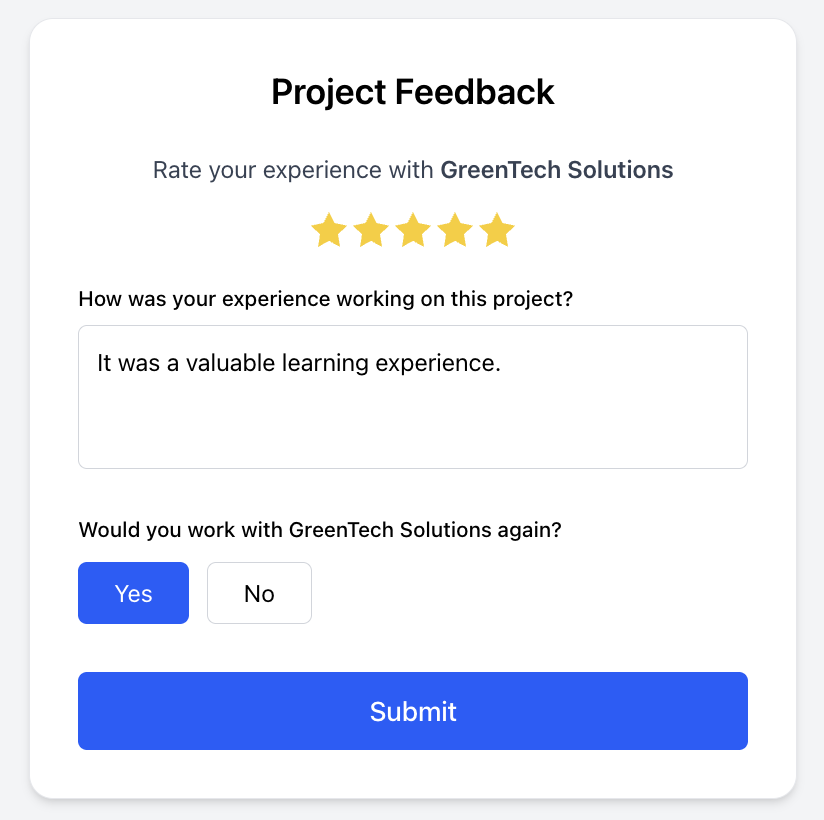
\includegraphics[width=0.8\linewidth]{figures/Student-Project-Feedback.png}
  \caption{Feedback screen mock up balancing qualitative notes and structured scores.}
  \label{fig:feedback-screen}
\end{figure}

Documentation practices complete the process. \textit{Metric definitions} are stored in a public wiki, \textit{SQL} files are kept in Git, and quarterly snapshots save the state of each \textit{KPI}. This approach ensures that the analytics remain reproducible and that future contributors stay responsible for using the same definitions \citep{Choudary2016}.
